\documentclass[conference]{IEEEtran}

\ifCLASSINFOpdf
\else
\fi

\usepackage{graphicx}
\usepackage[linesnumbered,ruled]{algorithm2e}
\newtheorem{example}{Example}

\begin{document}

\title{Causality Analysis using the Descriptive Power of the Social Web}


% author names and affiliations
% use a multiple column layout for up to three different
% affiliations
% \author{\IEEEauthorblockN{Michael Shell}
% \IEEEauthorblockA{School of Electrical and\\Computer Engineering\\
% Georgia Institute of Technology\\
% Atlanta, Georgia 30332--0250\\
% Email: http://www.michaelshell.org/contact.html}
% \and
% \IEEEauthorblockN{Homer Simpson}
% \IEEEauthorblockA{Twentieth Century Fox\\
% Springfield, USA\\
% Email: homer@thesimpsons.com}
% \and
% \IEEEauthorblockN{James Kirk\\ and Montgomery Scott}
% \IEEEauthorblockA{Starfleet Academy\\
% San Francisco, California 96678--2391\\
% Telephone: (800) 555--1212\\
% Fax: (888) 555--1212}}

\maketitle

\begin{abstract}
Social Web is a knowledge source which contains reasons behind events. For instance, tweets in Twitter can tell us the reason of a traffic jam-pack in part of a city. In this paper, we discuss two use-cases of exploiting the Social Web for Causality Analysis. Our use-cases come from our collaborations with aviation industry and trade. We propose {\sc Swey} framework, a generic approach to quickly derive reasons from the Social Web. We also discuss challenges and future directions of this novel research direction.
\end{abstract}

\IEEEpeerreviewmaketitle

\section{Introduction}
\label{sec:intro}
Nowadays there exists huge amount of user-generated content all around the Web \cite{moens2014mining}. They serve different aims such as wikis, blogs, tweets etc. Social Web is the infrastructure of this content which brings an opportunity for users to interact and express ideas. Wikipedia, for instance, hosts 5,155,355 English articles written and refined by users\footnote{\it https://stats.wikimedia.org/EN/Sitemap.htm}. Also Twitter receives around 500 million tweets per day\footnote{\it https://blog.twitter.com/2011/numbers}. Although the Social Web is often considered as an informal and unverified knowledge source, it has recently attracted recearchers in data analysis for {\em insight discovery}. For instance, Twitter is used in \cite{bruns2013towards} for Sentiment Analysis, in \cite{mathioudakis2010twittermonitor} for Trend Detection, in \cite{cameron2012emergency} for Crisis Management and in \cite{DBLP:conf/kdd/RitterMEC12} for Event Prediction.

In this paper, we propose a novel analysis paradigm, i.e., to exploit the Social Web for Causality Analysis. Social Web has a descriptive power to explain reasons behind events, because it contains discussions of thousands of users around those events. Hence an unsupervised approach to understand ``why an event has happened'', is potentially a look-up on the Social Web. The volume of the Social Web enables us to easily highlight causalities behind events. For instance, one can quickly understand what people around the world are talking at the current movement by using {\em Tendances} in Twitter or {\em Trending Events} in Facebook.

Our focus in this paper is on the following question: ``how to describe events using the Social Web?'' The definition of {\em event} is adapted from data analysis community, i.e., an event in data, or {\em data observation}. Data scientists interact with data in form of visual or textual elements. For instance, they analyze the amount of monthly precipitation in New York in bar charts or population density of the United States in heat maps. A data scientist may then ask for the causality behind any event during her data analysis process. Example \ref{ex:flight} considers a flight data analysis case.

\begin{figure*}[htpb]
\centerline{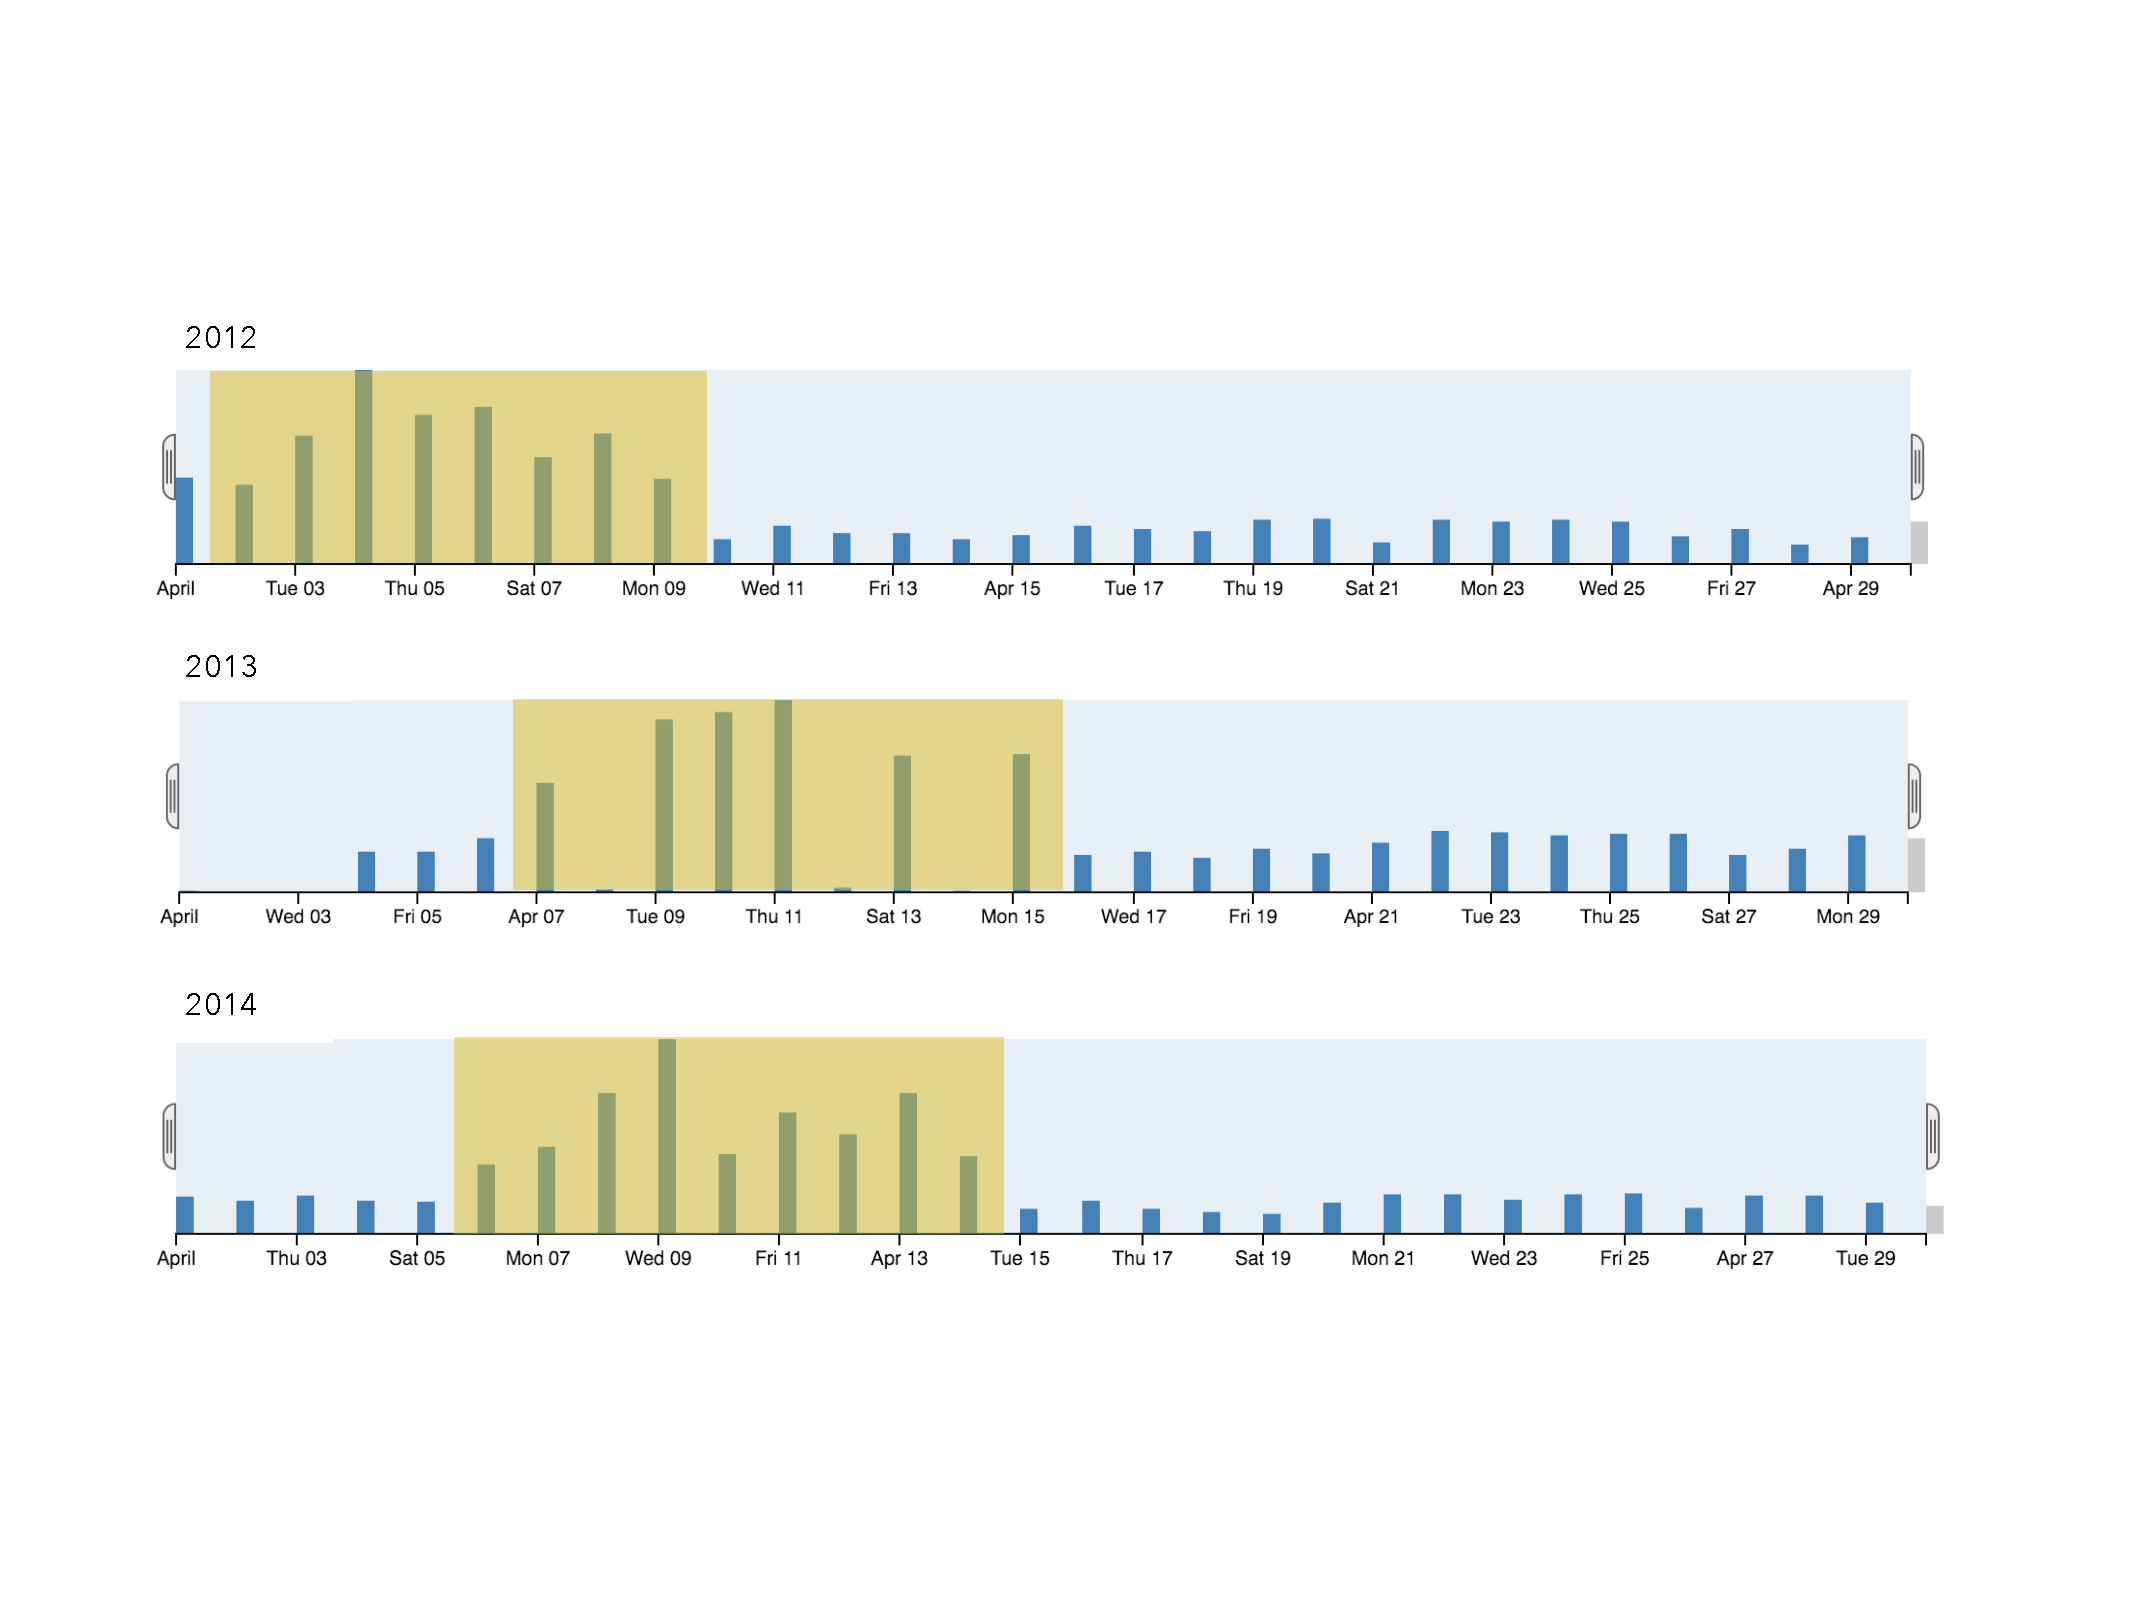
\includegraphics[width = .9\linewidth, keepaspectratio = true]{figs/ap12.pdf}}
\caption{\label{fig:ap12} Number of Flights Coming to Augusta Airport in Aprils of 2012, 2013 and 2014}
\end{figure*}

\begin{example}
\label{ex:flight}
Maria, a data scientist, is analyzing the number of flights during April 2012 landing in Augusta airport (Figure \ref{fig:ap12} top). She notices a drastic increase in number of flights during the first 10 days of April, but she doesn't know why. To know the reason behind this event, she decides to see what people are talking about in the Social Web during 10 first days of April 2012 in Augusta. For instance she can consider tweets published at that period of time and sent from Augusta. Frequent discussions in these tweets can potentially serve as explanations for the causality of the event. Maria observes that at that the most frequent discussion is ``Master's tournament'', i.e., a popular national event where a huge audience flies to Augusta for the event. Evidently, Maria concludes that the increase in number of flights is because of the sport event.
\end{example}

We believe that the Social Web can be employed for Causality Analysis from two different perspectives:

\begin{itemize}
\item Social Web describes an event to a {\em human}, i.e., human-centered Causality Analysis. In the literature, the focus has been always on this perspective. Example \ref{ex:flight} illustrates this case. In Section \ref{sec:human}, we present more details on this perspective by a use-case in aviation domain.
\vspace{5pt}
\item Social Web describes an event to a {\em machine}, i.e., machine-centered Causality Analysis. Often in a multi-layer system, two components cannot communicate with each other, because they follow different policies. Causality Analysis can be considered as a middle layer between these two components to explain input and outputs and make the hand-shaking process easier. As in Figure \ref{fig:machine}, an explanation for the input of the first component is given to the second one, instead of the its rough output. In Section \ref{sec:machine}, we present more details on this perspective by a use-case in trade domain. Notice although domain-specific ontologies can also be a solution for this case \cite{meij2011mapping}, but they are often not available or expensive to to construct.
\end{itemize}

\begin{figure}[htpb]
\centerline{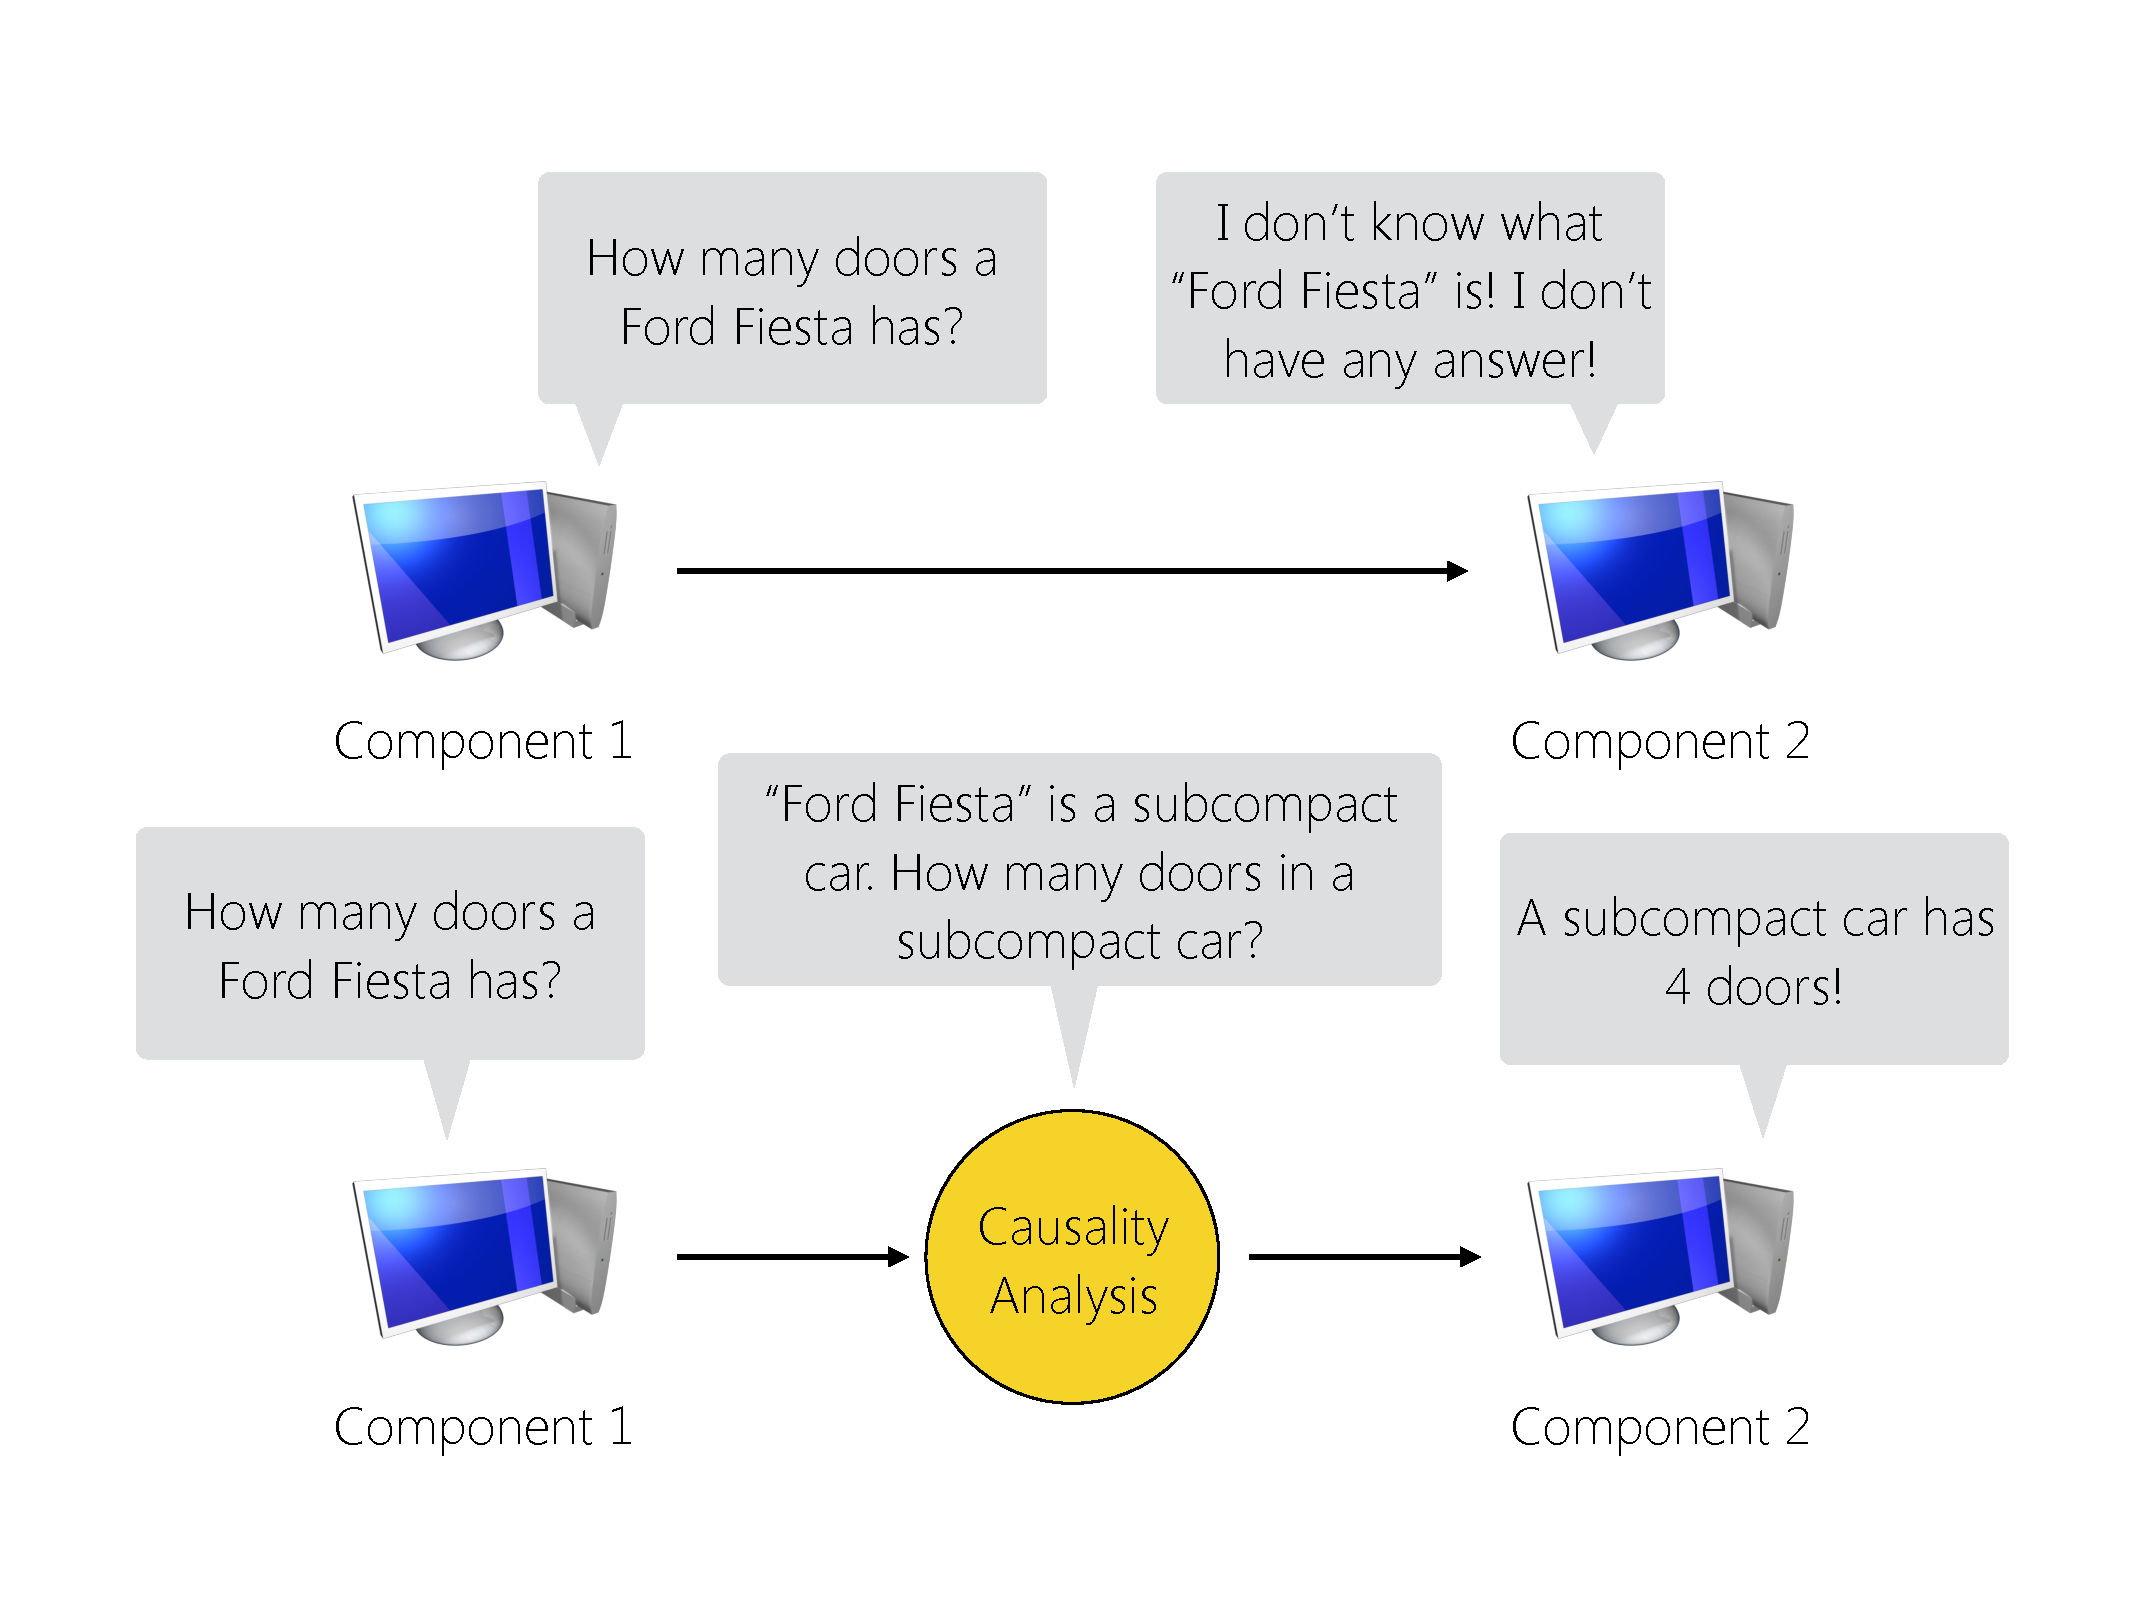
\includegraphics[width = 1\linewidth, keepaspectratio = true]{figs/machine.pdf}}
\caption{\label{fig:machine} An Example of Machine-centered Causality Analysis}
\end{figure}

Our use-cases in Sections \ref{sec:human} and \ref{sec:machine} are both verified by domain experts to see how effective the Social Web can contribute to Causality Analysis.\\

\noindent {\bf Context of Causality.} While causality analysis covers a large space of causes, we need to specify the context where we consider our problem. We are in an {\em ad-hoc} and {\em non-deterministic} context. Being ad-hoc means that there is no a-priori knowledge or no prior model about the cause of events. This is also called observational causality analysis in the literature. In other words, in an ad-hoc context, Causal Bayesian Network~\cite{li2015practical} is not available or known in advance. An event like ``observing smoke'' happens in an {\em versatile} context (and not ad-hoc) where we can consider some probable reasons that may have potentially produced smoke, e.g., ``lighting a cigarette'' or ``burning a food''. Also we adapt the non-deterministic context defined in Suppe’s causality: an event $X$ is a cause to the event $Y$ if

\begin{itemize}
\item $X$ occurs before $Y$;
\item likelihood of $X$ is non zero;
\item likelihood of occurring $Y$ given $X$ is more than the likelihood of $Y$ occurring alone.
\end{itemize}

While causality describes a {\em certain} reason behind an event, the most natural model employed in the state of the art is {\em probability models}. We also follow the literature \cite{hlavavckova2007causality} and adapt a probability model. 
%On top of the probability model, we also {\em quantify} results in order valorize probability results. The quantification process is described separately for both use-cases in their respective sections.
% Our main method for quantification is {\em Kullback–Leibler divergence} \cite{kullback1951information}.

The outline of this paper is as follows: In Section \ref{sec:proposal}, we present our proposal. Then in Sections \ref{sec:human} and \ref{sec:machine}, we illustrate two use-cases to shed light on two perspectives on Causality Analysis. In Section \ref{sec:discussion}, we mention some challenges and future improvements of our proposal. Last, we conclude in \ref{sec:conc}.

\section{SWEY Framework}
\label{sec:proposal}
We propose a framework called {\sc Swey} which is based on a simple intuition that {\bf S}ocial {\bf W}eb {\bf K}nows {\bf W}hy. Our proposal considers a simple observation, i.e., the knowledge derived form the Social Web can explain events which are hard or infeasible to be explained otherwise. We present two use-cases in subsequent sections where such knowledge can be exploited to make a {\em human} or a {\em machine} aware of the causality of an event. Algorithm~\ref{algo:swey} illustrates our Causality Analysis framework.

\begin{algorithm}
\DontPrintSemicolon
\KwIn{$k$, $\sigma$, Concepts ${\mathcal C}$}
\KwOut{Set of $k$ words ${\mathcal W}$}
${\mathit weighted\_bag} \gets 0$\;
\For{$s \in {\mathcal S}$}
{
  $words \gets {\mathit get\_words}(s, \sigma)$\;
}
\For{$word \in words$}
{
  ${\mathit weighted\_bag}[word] ++$\;
}
$sort({\mathit weighted\_bag})$ // on weights\;
${\mathcal W} \gets {\mathit weighted\_bag}[0,k]$\;
\Return{${\mathit weighted\_bag}$}\; 
\caption{SWEY Algorithm}
\label{algo:swey}
\end{algorithm}

The algorithm gets as input a set of concepts ${\mathcal C}$. Concepts are usually user-defined. 
% In case of spatiotemporal observation,  like the usecase in Section \ref{sec:human}, ${\mathcal C}$ is the temporal period and the location. In case of trader hub data, ${\mathcal C}$ is manually given by users.
The algorithm begins scanning all available sources ${\mathcal S}$, e.g. Wikipedia, Twitter, Facebook, Newsfeed, Forums, etc. In our use-cases we exploit Twitter and Wikipedia. Note that in our generic framework, we can use any number of sources. However, there are challenges associated to multi-source exploitation, which we discuss in Section \ref{sec:disc}.

The array $words$ keeps all words in every $s \in {\mathcal S}$. Then tuples of the form $\langle word, count\rangle$ are inserted into ${\mathit weighted\_bag}$ by counting number of occurrences of each word in $words$. Then we sort $words$ in descending order of weights and insert first $k$ words into ${\mathcal W}$, i.e., the output.

The complexity of this simple algorithm is ${\mathcal O}(|{\mathcal S}| + m \times log m)$ where $m = |words|$. Normally $m \gg |{\mathcal S}|$, hence the efficiency of the algorithm is heavily dependent of the content volume of sources. For that, we designed the ${\mathit get\_words}()$ function in a way that it scans and stores only necessary words. Some considerations for this function are as follows:

\begin{itemize}
\item The function employs a list of stop words and avoid scanning them;
\item Based on DOM\footnote{Document Object Model} structure, the functions scans only specific parts of an HTML page. For instance, it avoids scanning footers.
\end{itemize}

Not only we scan necessary words, we can sample words in random for more efficiency. This would be a precision lost in cost of performance. The trade-off between precision and performance can be tuned by the parameter $\sigma$ which is the sampling ratio. The parameter dictates to the algorithm to pick one word among $\sigma$ words at random. Obviously if $\sigma = 1$ no sampling occurs.
% In our usecases, we use $\sigma = 3$ in Section \ref{sec:human} and $\sigma = 1$ in Section \ref{sec:machine}. This way, both algorithms run instanly.

Next two sections present two use-cases for {\sc Swey} in two different domains, aviation and trade. The aim is to show how the Social Web can effectively contribute to Causality Analysis for humans and machines.

\section{Human-served Causality Analysis}
\label{sec:human}
We believe that Causality Analysis using the Social Web can be exploited to help humans understand reasons behind events. In this section, we present a spatiotemporal use-case in aviation domain.

Flight data contains abstract information about aircrafts, departure/arrival locations and times. It also contains detailed information about the location of flights in 3D space (latitude, longitude and altitude) by the precision of seconds or minutes. Flight data is often huge and hard to analyze. Our flight data is obtained from FAA (Federal Aviation Administration) which contains all flights from January 2012 to December 2014 inclusive. The data has around 4.5 billion records and takes around 45GB on disk. Each record corresponds to a location record of a flight. There exists one minute difference between the timestamps of two consequent records.


The volume of flight data, both vertically (number of records) and horizontally (number of attributes) makes the analysis of such data difficult. Recently {\em interactive visualization} methods have contributed a lot to flight data analysis \cite{lins2013nanocubes}. Visualization by its own is a useful method for any spatiotemporal dataset to illustrate characteristics and correlations inside data. But the challenge for such methods is that they usually don't scale to huge volume of flight data. Moreover, an aviation expert is usually interested to quickly look at different aspects of data with different zoom levels. So she needs to query on visualization iteratively. Often visualization techniques are unable to respond to the fast rate of queries coming from experts. Because each query execution needs a screen refresh which means redrawing all graphical elements. This is a time-consuming process. Interactive visualization techniques is a solution by following considerations:

\begin{itemize}
\item {\bf Backend}. First in backend, different methods like speculative exploration \cite{DBLP:conf/icde/KamatJTN14}, caching, indexing, etc. help to boost the performance. These techniques are applied on new data structures which make the data access more efficient.
\vspace{5pt}
\item {\bf Frontend}. Following backend structure, some optimizations are done during execution in frontend. For instance, visual computations are limited to number of available pixels on the screen, or queries don't lead to redraw the visualization but only update the differentiated part.
\end{itemize}

\begin{figure*}[htpb]
\centerline{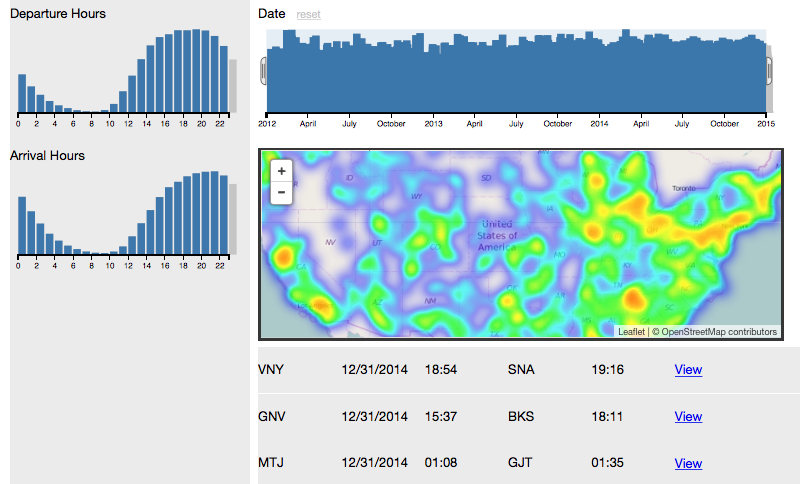
\includegraphics[width = .8\linewidth, keepaspectratio = true]{figs/spacetime.png}}
\caption{\label{fig:spacetime} FAA Visualization Tool}
\end{figure*}

We built a visualization framework for FAA from the scratch by inspiring from the state of the art. This specific visualization tool corresponds to the needs of FAA. Figure \ref{fig:spacetime} illustrates one screen-shot of this tool. Among many different dashboards that we made available for the FAA aviation experts, here we focus on one dashboard, i.e., {\em multi-flight visualizer}. In this dashboard, the expert can specify desiderata to visualize a desired subset of flights. Then as in Figure \ref{fig:spacetime}, the multi-flight visualizer shows different aggregations of the subset:

\begin{itemize}
\item {\bf Histograms.} Histograms for number of flights per departure/arrival hour and date are shown. By looking at these histograms, an expert can quickly understand when (which hour or which date) and increase/decrease in number of flights have occurred.
\item {\bf Heatmap.} It shows the geographical concentrations of flights over the US map. By looking at this histogram, the expert can quickly understand which part of the US is more concerned regarding her intended subset.
\item {\bf Table.} In a column/row-format table, information about actual flights in the intended subset are shown. Information contains departure/arrival locations and times.
\end{itemize}

The most important functionality in multi-flight visualizer is {\em interactivity}. The expert can brush on any histogram and filter her selection. This way, all other visualization components (other histograms, heatmaps and tables) will be automatically updated to reflect the filtered data. Note that this action is done immediately. This enables experts to quickly look at different aspects of the data.

We present a running example which clearly shows our use-case. Nina, an aviation expert, is analyzing flights coming to Augusta airport in April 2012. She finds that there is a sudden increase in number of flights in the first 10 days of this month (Figure \ref{fig:ap12} top). To see whether this is a random observation or not, she decides then to look at flights coming into Augusta airport in April 2013 (Figure \ref{fig:ap12} middle). In this new subset of flights, she also finds out an increase between April 7 and 15. Now her hypothesis is that there is an annual pattern for an increase in number of flights in month of April. She is interested to discover the reason behind this pattern. This is important for Nina to know the reason behind this increase, because it makes planning difficult, hence user satisfaction (regarding airlines and airports) decreases drastically. If Nina finds out the reason behind this increase, she can plan in advance for next occurrences of that event. This is how Causality Analysis is beneficial for an aviation expert.

For this aim, Nina runs {\sc Swey} by providing following concepts: ``April 1-10 2012'' and ``Augusta''. For this use-case, {\sc Swey} uses Twitter as the only source. {\sc Swey} retrieves tweets if they satisfy both following conditions:
\begin{itemize}
\item Tweet should be posted during April 1 to 10, 2012;
\item Tweet should be sent from Augusta.
\end{itemize}

\begin{figure*}[htpb]
\centerline{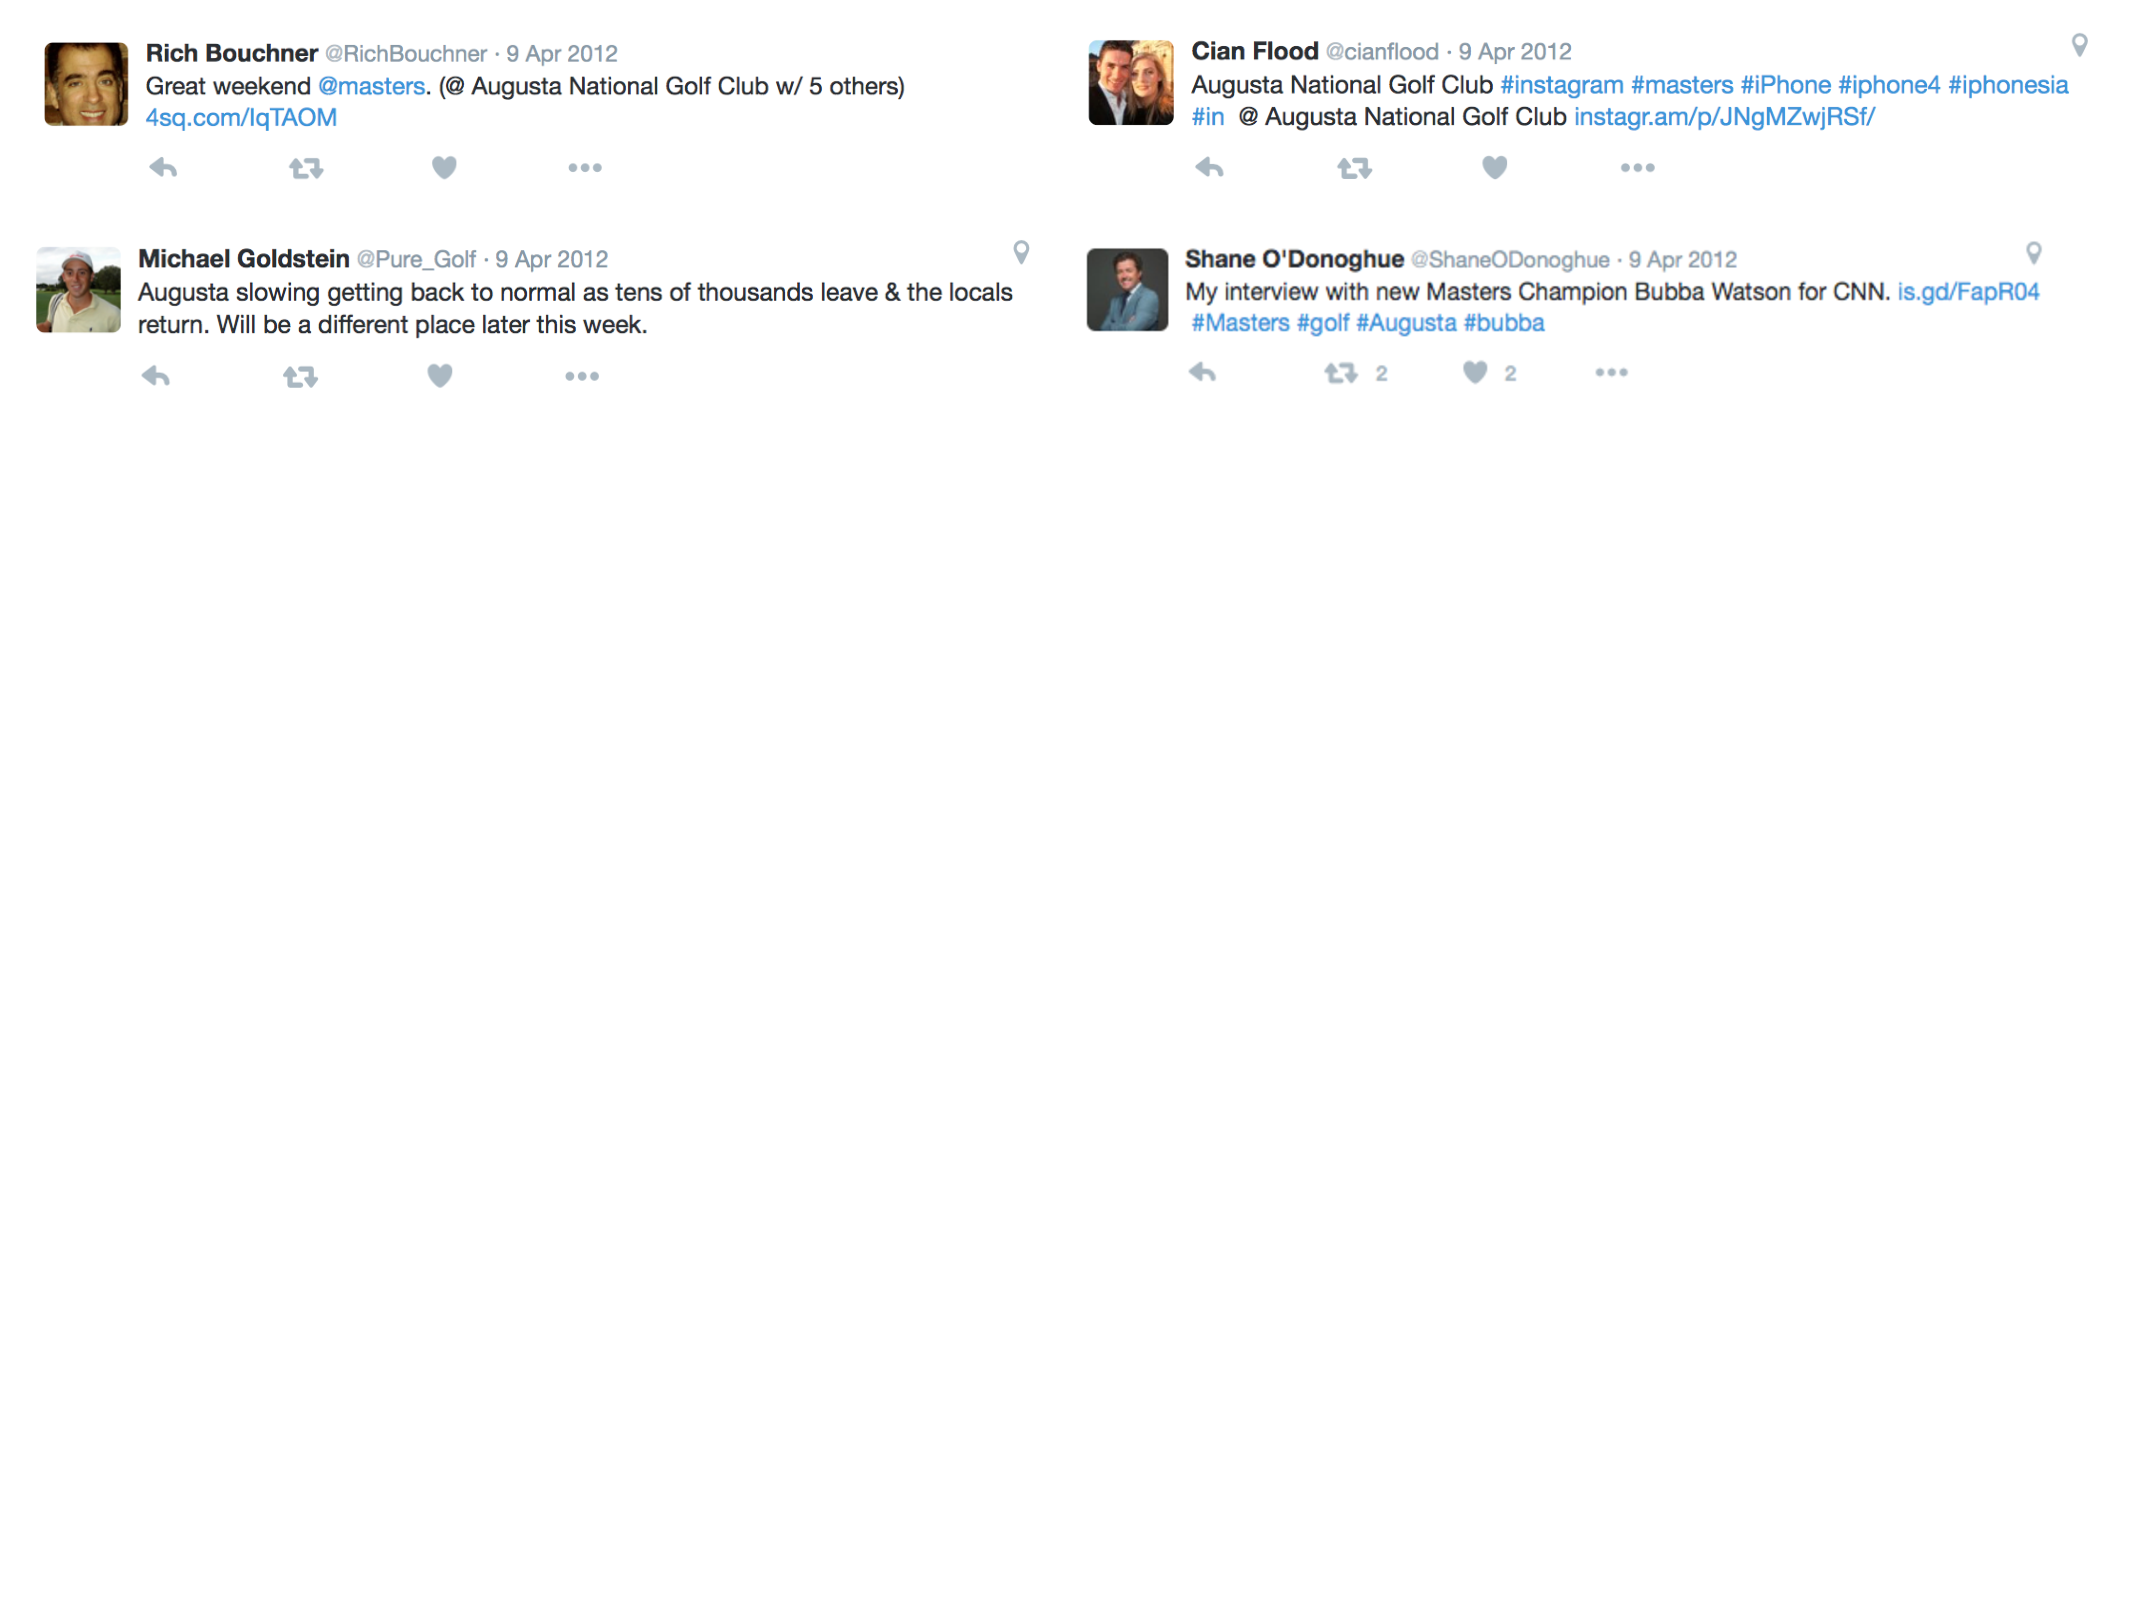
\includegraphics[width = 1\linewidth, keepaspectratio = true]{figs/tweet.pdf}}
\caption{\label{fig:tweets} Instances of Tweets between April 1-10, 2012 in Augusta}
\end{figure*}

Some retrieved tweets are shown in Figure \ref{fig:tweets}. Following Algorithm \ref{algo:swey}, next the system will generate a weighted bag of words using all words appeared in the set of tweets. Weighted bag keeps each words and number of its occurrences, i.e., its frequency. Then the system reports top-$k$ words to the experts. In this example, we consider $k = 5$. Hence, Nina receives following 5 words in descending order of appearance: ``masters'', ``results'', ``winner'', ``finisher'', ``tournament''. Nina can easily conclude the reason behind the event in two following ways.

\begin{itemize}
\item {\bf Abstract View}. The reason behind the increase in number of flights strongly relates to an {\em sport} event (by considering words like ``results'', ``winner'', ``finisher''). 
\item {\bf Precise View}. The reason is the Masters Golf tournament, which has happened in Augusta between April 5-8, 2012. It is a national event and many people from different parts of the country reach Augusta to watch the tournament.
\end{itemize}

While Nina is now sure that the reason behind the increase is Masters tournament, she wants to do the same process for the year 2013. Executing {\sc Swey} for April 7-15, 2013 returns following results: ``masters'', ``golf'', ``results'', ``tournament'', ``scott''. There exits 3 common words between the results of 2012 and 2013 and Nina is now confident that the reason behind the increase in both years is Masters tournament. Some side observations are as follows:

\begin{itemize}
\item Note the order of top-$k$ words in both results: the word ``masters'' appears in the first position. This means that this word has the strongest correlation with the event.
\item We already discussed that Causality Analysis can be seen in two different detail levels, abstract and precise. It is possible that for a use-case, no specific word like ``masters'' is returned. In this case, {\sc Swey} can still provide an abstract view.
\item Although the term ``tournament'' is expected to be highly correlated with the event, it appears almost at the end of both lists. The reason is that our knowledge source is Twitter, i.e., an informal source. Users in Twitter tend to use familiar words rather than official. For instance, we observe that the concept ``tournament'' is addressed with other words like ``winner'' or ``finisher''.
\item Although the reason behind the increase in number of flights is Masters tournament for both years, the set of top-$k$ words contains some different words for different years. This opens up a a novel perspective view which we call {\em Side View} where we get a sense of focuses around the main event. For instance, in our example, it shows that in 2013, people are very excited about the fact that ``Adam Scott'' has been the winner. 
\end{itemize}

The last question is on usability of Causality Analysis: now that Nina knows the reason behind the increase in number of flights for two consecutive years, can she use such information to predict events for 2014? Masters tournament in 2014 happened between April 10 and 13. Nina analyzes the distribution of flights in April 2014, as shown in Figure \ref{fig:ap12} bottom. She clearly observes a drastic increase around that period. This clearly means that she can exploit Causality Analysis results to predict events in the future and for planning in advance.

\section{Machine-served Causality Analysis}
\label{sec:machine}
We believe that Causality Analysis using the Social Web can even be exploited to describe events to machines. A common case is when two components cannot communicate with each other because their inputs and outputs do not match (Figure \ref{fig:machine}). In this section, we discuss a use-case in {\em unofficial-to-official} context: an expert queries formal databases (e.g., laws) with informal words and this normally leads no response. Our use-case is in trading domain.

In international trading, one important concept is landed cost of imported/exported products. This mainly refers to taxes, transport and monitoring costs. Around 190 countries use a universal standard called HS\footnote{Harmonized Commodity Description and Coding System: http://www.wcoomd.org/en/topics/nomenclature/overview/what-is-the-harmonized-system.aspx} to define this cost for any possible trading product. In this system, any product is identified with a HS code under a specific hierarchy. For instance, the HS code for ``fresh potato'' is $0701.90$ and it is under the category of ``Potatoes, fresh or chilled'' and sub-category of ``other''. The HS standard has been constructed and maintained by the World Customs Organization (WCO) in Belgium. HS is based on an economic logic. For instance all products related to animals are placed close to each other in the HS hierarchy, while machinery and mechanical appliances are placed in another branch. 
 
The process of assigning an HS code to a product is called {\em HS Classification}. The assignment is based on a variety of factors like product's composition, form and function. Traditionally this task is done using trading lawyers who are HS experts. This is obviously an expensive task both monetarily and timely. An alternative solution is HS online classification systems (HOC). From the data analysis perspective, HOC is an advanced search engine over the formal data of HS codes. HOC begins with an input query from the user. Then it verifies the query against HS codes. This results in a candidate set of HS codes. Then HOC asks questions to disambiguate between candidates to finally land on one target HS code. One example HOC is the one for Nigeria Trading Hub Classification System\footnote{http://www.nigeriatradehub.gov.ng}.

\begin{figure*}[htpb]
\centerline{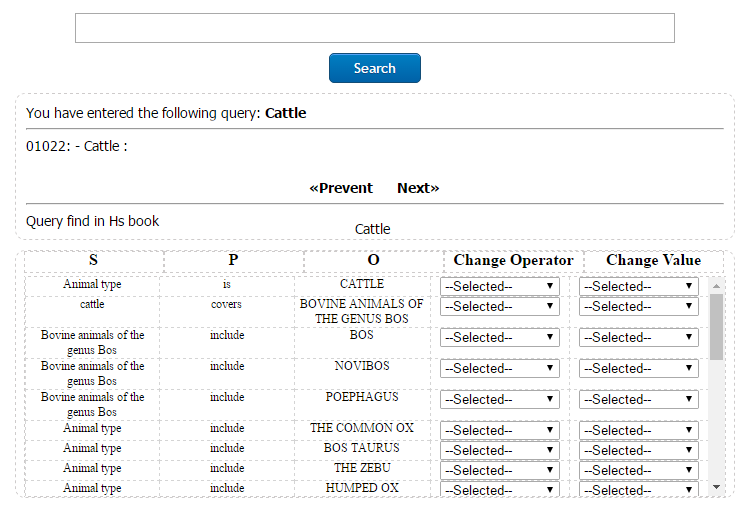
\includegraphics[width = .8\linewidth, keepaspectratio = true]{figs/claxper.png}}
\caption{\label{fig:claxper} Showing HOC Results for the Query ``Cattle''}
\end{figure*}
 
Most HOC systems are proprietary. We designed an open-source HOC based on {\sc Swey} which provides HS codes for queries based on HS standard descriptions. Figure \ref{fig:claxper} illustrates a screenshot of our HOC searching for the query ``Cattle''.

However in a HOC system, there may be queries with no result. An example is Figure \ref{fig:machine} top. In general, if query terms are never mentioned in HS descriptions, there is no chance to find an appropriate HS code. This is the {\em status quo} of all current HOC systems. That means a typical HOC stops at the point where the query returns no results. For instance, in Figure \ref{fig:hs} left, the expert enters the query ``Ford''. Basically, no result can be returned for this query because this term has been never mentioned in HS descriptions. But if the system knows that {\em Ford is in fact a car}, then an appropriate HS code for the term ``car'' can be simply returned. This is the motivation behind {\em Background Search} functionality in our HOC. 

\begin{figure*}[htpb]
\centerline{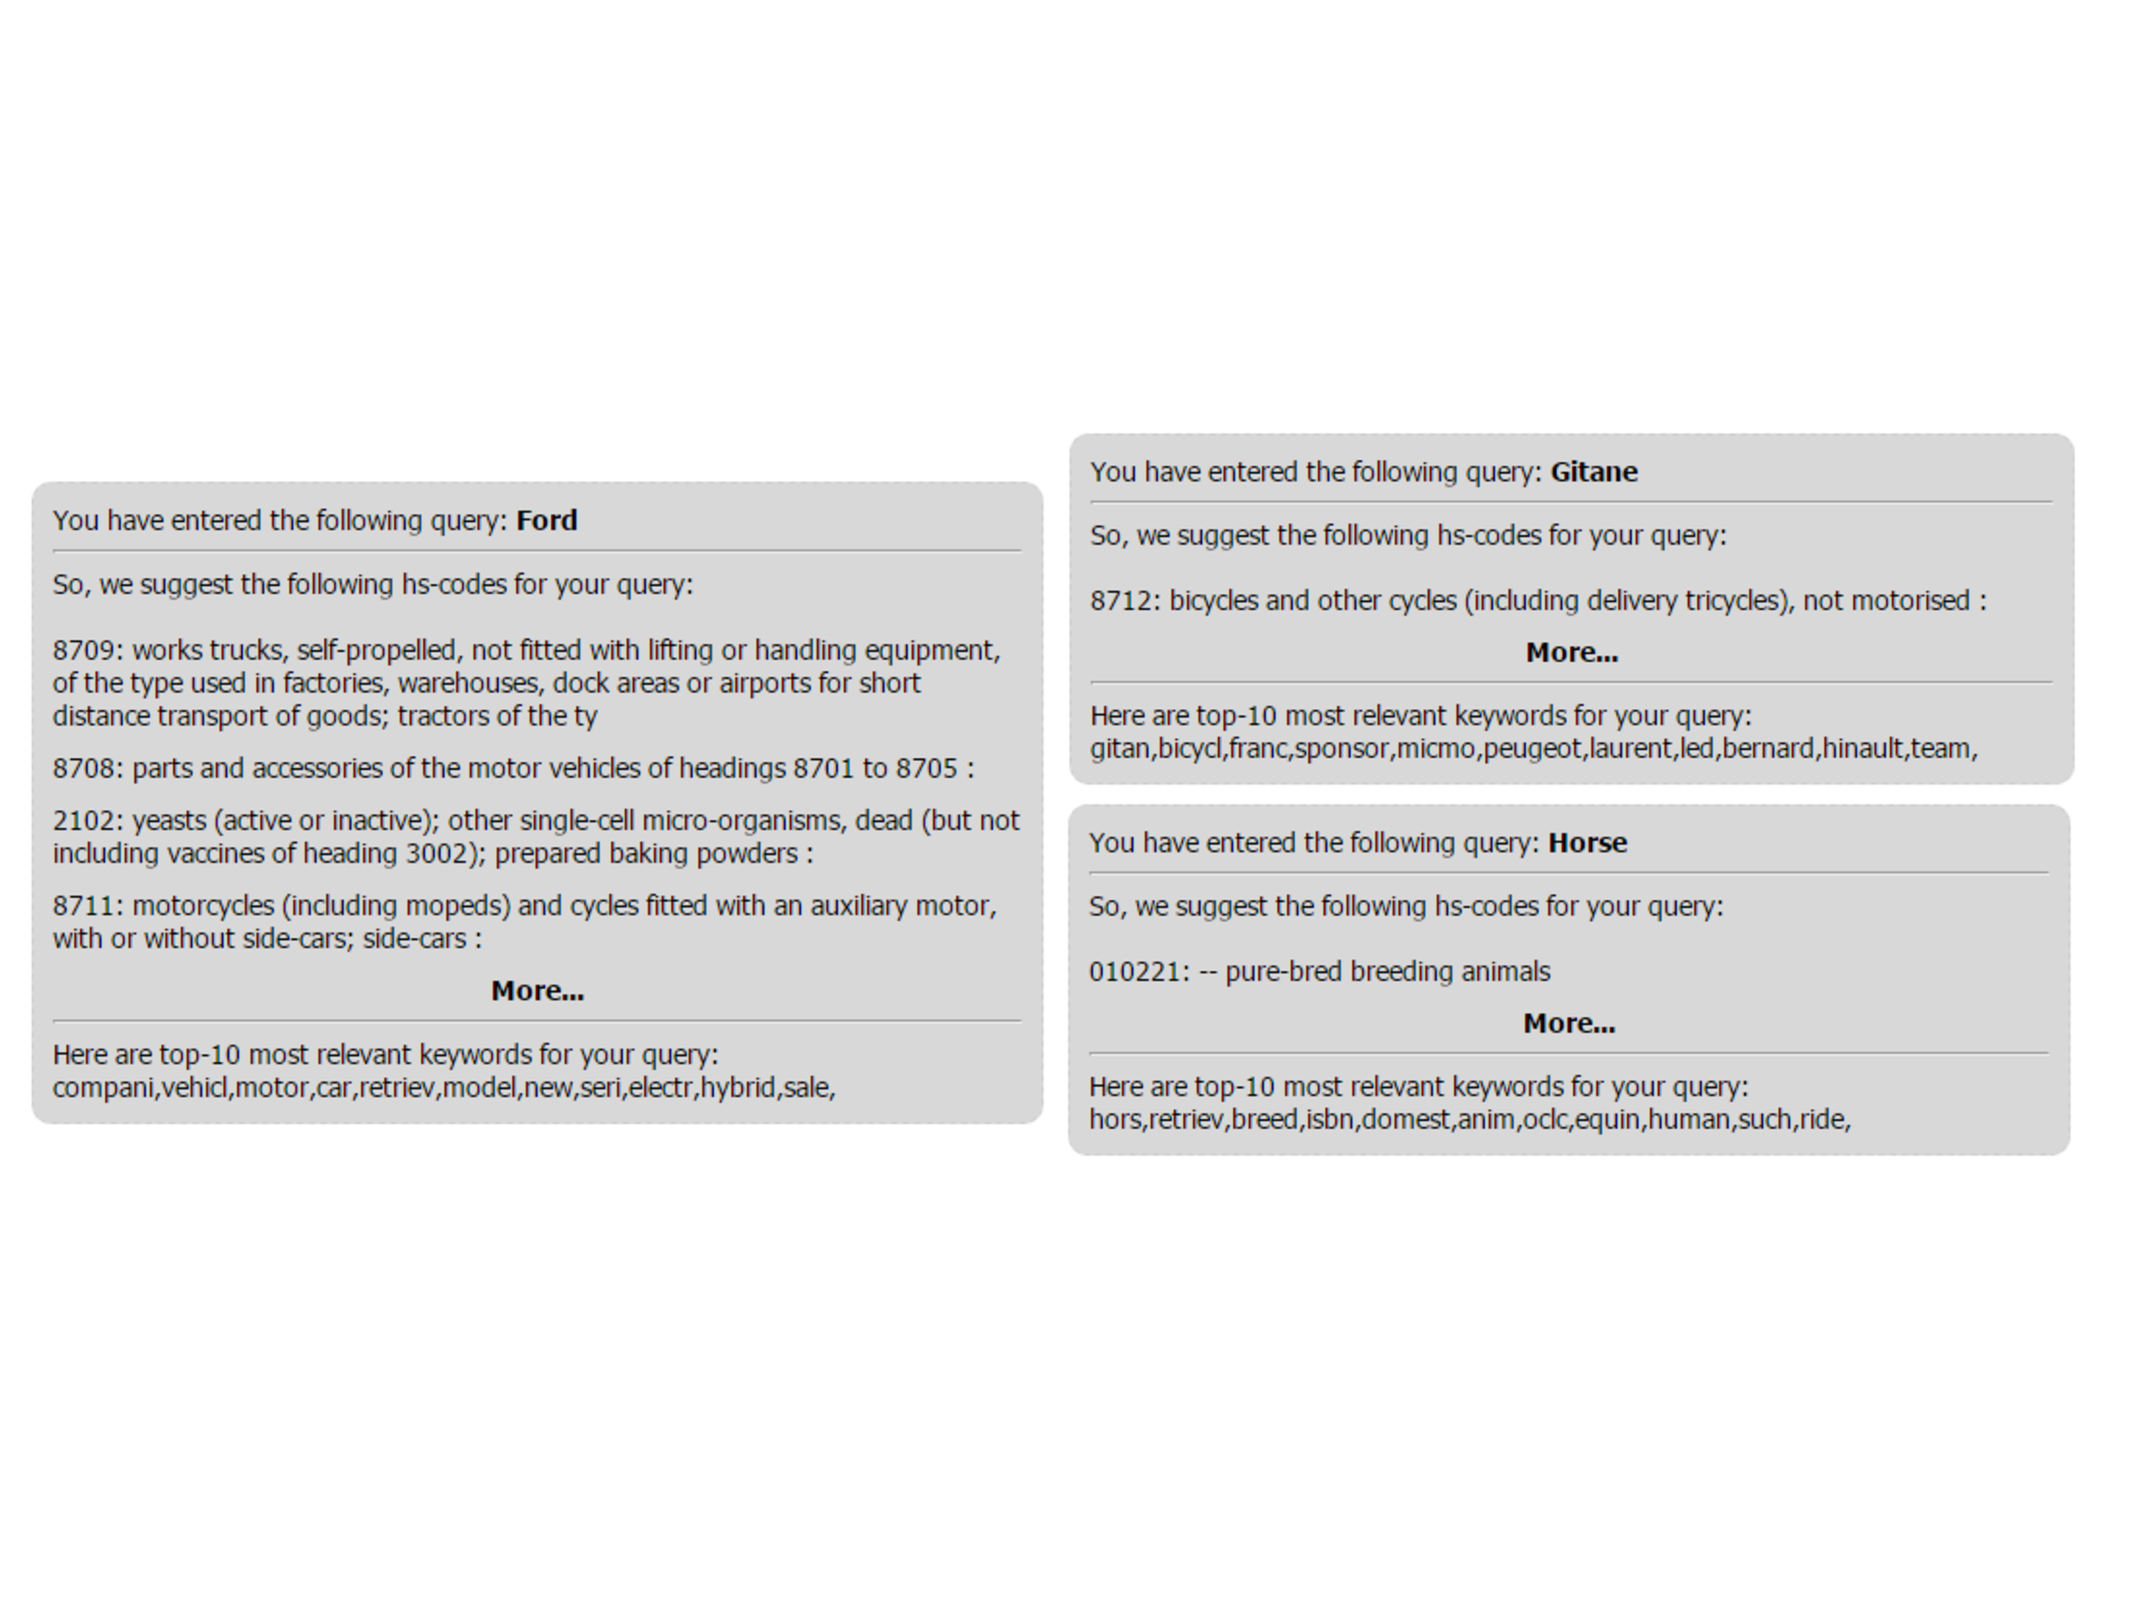
\includegraphics[width = .8\linewidth, keepaspectratio = true]{figs/hs.pdf}}
\caption{\label{fig:hs} Background Search Results}
\end{figure*}

Background Search is the adaptation of {\sc Swey} using Wikipedia as knowledge source for an HOC. It is a Causality Analysis component which explains the input query to the search engine using the Social Web. In the absence of result for an input query (like queries in Figure \ref{fig:hs}), Background Search finds a list of co-occurring words with input query from Wikipedia and queries HS descriptions using top-10 frequent words obtained from the knowledge source. Background Search employs stemming algorithms \cite{jones1997readings} to avoid separate counts for variants of a single word (e.g. community and communities). Table \ref{tbl:bg} illustrates some results of Background Search from different categories.


\begin{table}
\centering
\begin{tabular}{|c|c|c|}
\hline
{\bf Category} & {\bf Query}  & {\bf Result} \\ \hline
Brand & Toyota & Motor, Vehicle, Car,\\
& & Hybrid, Japan, Sale\\ \hline
Animal & Kitten & Cat, Mother,\\
& & Domestic, Short-hair\\ \hline
Food & Entrecote & Steak, Fillet, Cut,\\
& & Beef, French, Restaurant\\ \hline
Medicine & Paracetamol & Acetaminophen, DOI, Pain,\\
& & Drug, Liver, Acid\\ \hline
Person & Obama & Barack, President, States\\ \hline
\end{tabular}
\caption{Background Search Results}
\label{tbl:bg}
\end{table}


\section{Discussion}
\label{sec:discussion} 
We verified the usability of both usecases mentioned in Sections \ref{sec:human} and \ref{sec:machine} in different sessions with aviation and trading experts, respectively. Most of the experts appreciated the way they can immediately find out reasons behind observations. Examples used in this papers are some picks of experts' usage. However, this generic idea of causality analysis has a long way of improvement. Two immediate directions are {\em ontology-based analysis} and {\em user feedback}.

\vspace{5pt}
\noindent {\bf Ontology-based Analysis}. We already mentioned the difference in the literature used in the Social Web as an informal source compared to formal sources. Although looking for causality on the Social Web has promising results, but it cannot always fully answer queries. This is why one of our future works is using an ontology instead of the Social Web. DBPedia in an online public ontology of Wikipedia content. So our immediate improvement is to think of an SPARQL\footnote{SPARQL is the query language on ontologies} meta-query on DBPedia to be replaced by current HTML-lookup on Wikipedia pages. Ontologies enable a search over a structured space where relations between concepts are known in advance.

\vspace{5pt}
\noindent {\bf User Feedback}. Our {\sc Swey} framework can benefit a lot from user feedback. Our immediate direction is to exploit user feedback for the multi-source problem: Iterating over different sources may make the algorithm slow. On the other hand, all sources do not have the same quality and usefulness for an intended query. A solution to this problem is to pick sources in random in a weighted-lottery fashion. A source which has already received a higher appreciation (though user feedback) is more probable to be picked for the next round of scanning sources. Once results are shown to the analyst, the expert provides a feedback which reflects his/her appreciation. This way we update weights for each source to be used in the lottery process.

\section{Conclusion}
\label{sec:conc}
In this paper, we motivated the fact that the Social Web can be a strong knowledge source to explain data events. We discussed two sides of Causality Analysis for humans and machines. We proposed {\sc Swey} framework and discussed its functionality. Last, we presented challenges and future directions of this line of work.

\bibliographystyle{abbrv}
\bibliography{main}


\end{document}


